\documentclass{article}
\usepackage{amsmath}
\usepackage{graphicx}
\usepackage{multirow}
\usepackage{natbib}
\usepackage{caption}
\usepackage[margin=1in]{geometry}
\begin{document}
        
\title{Credit Balance MLR}


\author{Greg Sadler and Jackson Curtis}
\maketitle 

\section{Introduction}

One of the ways credit card companies make money is by credit card users accruing interest on their monthly balance. However, users who run high balances frequently face bankruptcy, which results in a significant loss to the credit card company because they have to write off the balance. Therefore, the credit company's ideal customers carry a medium balance with low risk of bankruptcy. 

Because of this, credit card companies are interested in being able to estimate the balance a customer will carry based off other information they have on the customer. This estimate could be used predictively in the credit card approval process (where customers are given cards only if they are likely to be a profitable customer) or descriptively, where the company uses what they learn about customers with medium balances to target advertising towards people with those same characteristics. Our analysis will address both these questions.

The dataset we have been given contains the monthly balance of customers, along with ten explanatory variables. We will learn about the explanatory variables by performing multiple linear regression with balance as our response variable. This will allow us to obtain estimates for the effects of the explanatory variables, predictions for future observations, and uncertainty estimates for both.

\section{Data Exploration}
We'll start by exploring the data we have been given and make sure that it meets the assumptions of multiple linear regression. The data set consists of 294 individuals with 11 observed variables and no missing data. Four variables (gender, ethnicity, marital status, and student status) are categorical while the rest are quantitative.
\begin{figure}
\centering
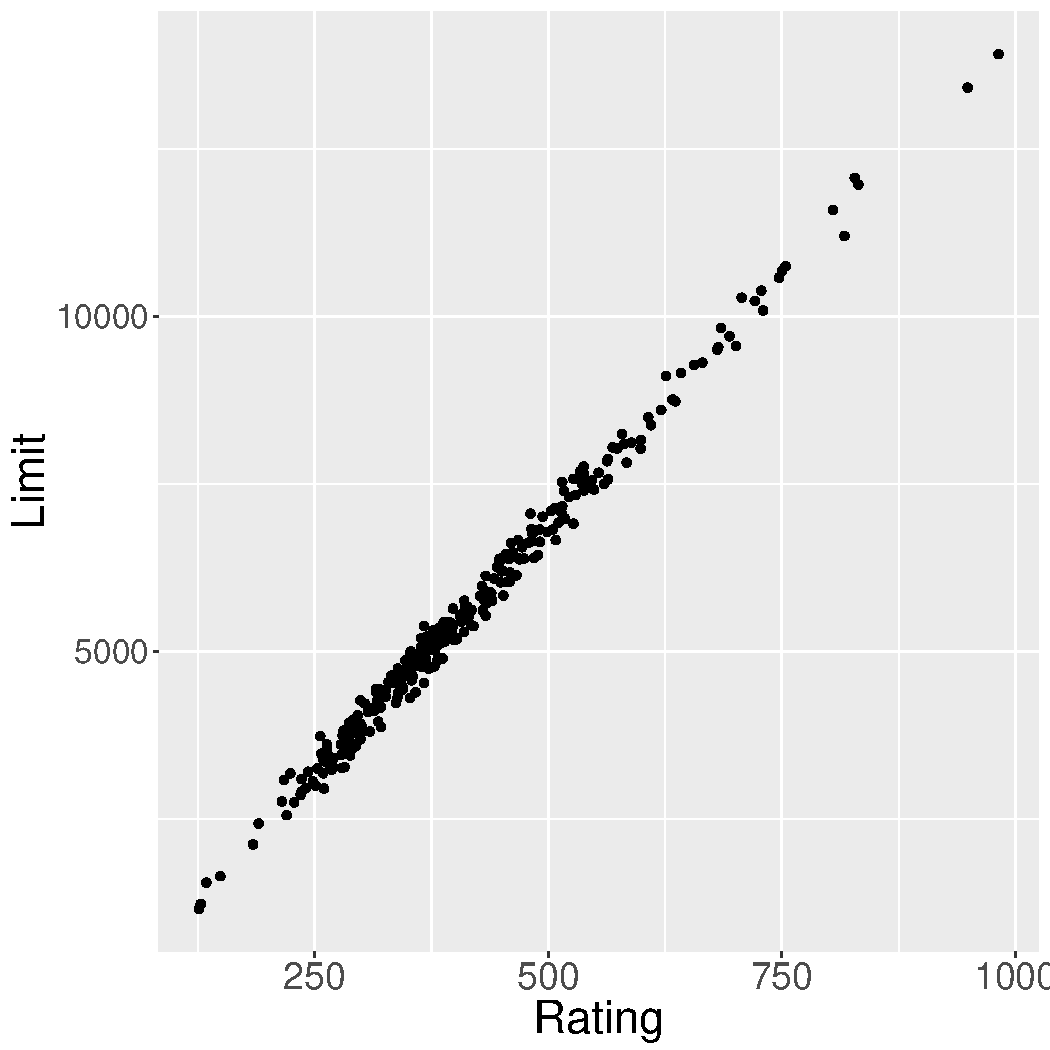
\includegraphics[scale=.3]{limitRating.pdf}
\caption{Credit limit and rating are highly collinear. }
\label{lr}
\end{figure}
One concern in that data is shown in Figure \ref{lr}. Credit rating and credit limit are highly correlated, so much so that it is reasonable to infer that credit limits are assigned based solely off rating. It is likely unnecessary to include both variables in our model since they contain the same information, and unwise because they will cause instability in our parameter estimation.


\begin{figure}
\centering
\includegraphics[scale=.5]{AVplot.pdf}
\caption{Added variable plots for all quantitative variables. }
\label{av}
\end{figure}

The added-variable plots in Figure \ref{av} help validate our model assumptions as well as show which variables have the strongest relationship with monthly balance. The plots were created using all variables except credit limit in order to capture the true effect of credit rating. All the plots show that the linearity assumption for the relationship between the explanatory variable and the response is well justified. In addition, we don't see strong evidence of heteroskedastic data (data in which the variance is different based on the magnitude of x).  
\section{Model Selection}
something about AIC best subset selection
And how we looked at the interaction and decided it wasn't significant

Our final model can be written as:

\begin{equation}
Balance = \beta_0+ \beta_1 * Income + \beta_2 * Limit + \beta_3 * Cards + \beta_4 * Age +\beta_5*Student +\epsilon
\end{equation}
$$\epsilon \sim N(0, \sigma^2)
$$          

Where $\beta_0$ is our intercept, the other $\beta$s are the effects for the explanatory variables, and $\epsilon$ are the residual errors.

\begin{table}
\centering
\begin{tabular}{|lrr|r|}
  \hline
 & DC & Marvel & Proportion \\ 
  \hline
Warner Brothers &  18 &   0 & 0.28\\ 
  Buena Vista &   0 &  10 & 0.16\\ 
  Fox &   0 &  14 &0.22\\ 
  Lionsgate &   1 &   2&0.05 \\ 
  New Line &   0 &   3 &0.05\\ 
  Paramount &   0 &   4& 0.06 \\ 
  Sony &   2 &   7 &0.14\\ 
  Universal &   0 &   3  & 0.05\\ 
   \hline
   Proportion & 0.33 & 0.67 &1\\
   \hline
\end{tabular}
\caption{Counts for studio and franchise for movies in dataset}
\label{combotab}
\end{table}


\end{document}